\documentclass[nostrict]{szablonPG}

%-------------------- Dodatkowe pakiety ---------------------
\usepackage{listing_schemat}
\usepackage{fourier}
\usepackage{polski}
\usepackage{setspace}
\usepackage{indentfirst} 
\usepackage{geometry}
\usepackage{graphicx}
\usepackage{subfig}
\usepackage{caption}
\usepackage{float}
\usepackage{enumitem}
\usepackage{wrapfig}
\usepackage{booktabs}
\usepackage{bigstrut}
\usepackage{siunitx}
\usepackage{amsmath}
%------------------------------------------------------------

%------------- Numeracja wzorów, tabel i obrazów ------------
\numberwithin{figure}{chapter}
\numberwithin{table}{chapter}
\numberwithin{equation}{chapter}
%------------------------------------------------------------
%			      Początek pracy dyplomowej  
%------------------------------------------------------------

\begin{document}

%------------------------------------------------------------
%  Dodanie strony tytułowej wygenerowanej z MojaPG oraz 
%  						oświadczenia


\includepdf{meta/strona_tytulowa.pdf}

\includepdf{meta/oswiadczenie.pdf}

%------------------------------------------------------------
%  Dodanie streszczenia i abstract
%  						

\chapter*{Streszczenie}
\indent Praca skupia się na aspektach automatyzacji diagnostyki działania laserowego tomografu komputerowego. Wraz z opisem budowy i zasady działania LCT przedstawiono w niej fizyczne aspekty działania akcelerometrów i żyroskopów, na których ma bazować opracowywany prototyp czujnika ze sterownikiem. Opisano również zagadnienie filtru Kalmana oraz zasadność jego wykorzystania w proponowanym rozwiązaniu. Następnie przedstawiono założenie i działanie platformy Arduino oraz modułu SEN0142, a następnie opisano tryb komunikacji pomiędzy poszczególnymi elementami opracowywanego urządzenia, tj.: komputerem z systemem \emph{Microsoft Windows}, Arduino, a modułem z akcelerometrem i żyroskopem.

\indent W dalszej części pracy przedstawiona została stworzona aplikacja, jej wygląd, funkcjonalności i ograniczenia, wraz z kluczowymi fragmentami kodu. Przytoczony został również skrypt samego sterownika (Arduino), który implementuje uprzednio opisane wzory.

\indent Następnie w pracy przedstawiono pomiary wykonane czujnikiem dla różnych położeń, na podstawie których możliwe jest określenie niepewności pomiarów. Wykazano również, że opracowane rozwiązanie nie sprawdza się w przypadku badań dynamicznych. Fakt ten zostaje poddany dalszej analizie.

\indent W podsumowaniu przedstawiono przykładowe propozycje rozwiązań mające na celu zarówno ulepszenie, jak i naprawę działania urządzenia.
\vspace{0.5cm}\newline
\textbf{Słowa kluczowe:} wzorcowanie, akcelerometr, kąty RPY
\vspace{0.5cm}\newline
\noindent \textbf{Dziedzina nauki i techniki, zgodnie z wymogami OECD:} nauki inżynieryjne i techniczne, inżynieria biomedyczna

\chapter*{Abstract}
\indent The project focuses on aspects of automating the diagnostic performance of a laser-based tomograph. After a description of the LCT, the physical aspects of accelerometers and gyroscopes on which the prototype sensor with controller is based are presented. The Kalman filter is also addressed, and why its use is needed. Next, the premise and operation of the Arduino platform and the SEN0142 module are introduced. The next section presents the appearance of the sensor, and the communication between the various components of the device under development is also described, i.e.: the computer with the \emph{Microsoft Widnows} system, Arduino, and the module with the accelerometer and gyroscope.

\indent The next chapter is devoted to the created application, its appearance, functionalities and limitations, along with key code snippets. The script of the controller itself (Arduino), which implements the previously described designs, is also cited.

\indent The paper then presents measurements made with the sensor for various positions, from which it is possible to determine the uncertainty of the measurements. It is also shown that the developed solution does not work for dynamic tests. This fact is further analyzed.

\indent In conclusion, sample ideas for both improving and repairing the device's performance are presented.
\vspace{0.5cm}\newline
\textbf{Keywords:} calibration, accelerometer, RPY angles \vspace{0.5cm}

%------------------------------------------------------------
%	Utworzenie spisu treści pracy dyplomowej
\tableofcontents

%------------------------------------------------------------
%	Dodanie wykazu ważniejszych skrótów i oznaczeń 
\chapter*{Wykaz ważniejszych oznaczeń i skrótów} 
\addcontentsline{toc}{chapter}{Wykaz ważniejszych oznaczeń i skrótów}

\noindent LCT - laserowa tomografia komputerowa (laser computed tomography), \\
MEMS - mikroukład elektromechaniczny, \\
ADC - przetwornik analogowo-cyfrowy (analog to digital converter), \\
RPY - roll $\phi$, pitch $\theta$, yaw $\psi$: kąty eulerowskie względem osi (OY, OX, OZ)

%------------------------------------------------------------
%	Dodanie rozdziałów pracy dyplomowej - główne ciało dokumentu 

\chapter{Wstęp i cel pracy} 

Laserowy tomograf komputerowy to innowacyjne urządzenie opracowywane i udoskonalane w ramach szeregu projektów naukowych poświęconych dozymetrii wielowymiarowej wysokiej rozdzielczości na Wydziale Fizyki Technicznej i Matematyki Stosowanej PG. W \cite{algo} przedstawiono w postaci schematu blokowego proces pozyskiwania oraz przetwarzania obrazów w celach radioterapeutycznych. Dodanie do niego symulacji LCT jeszcze bardziej rozbuduje istniejący algorytm postępowania, ale umożliwi porównanie rozkładu dawki w przestrzeni trójwymiarowej otrzymanej w ramach symulacji z teoretycznymi oczekiwaniami wyliczonymi przez odpowiedni algorytm (bazujące na wokselach, jeżeli do diagnostyki zastosowano metodę SPECT/CT, to metody niesztywne rejestracji obrazów przyczyniają się do poprawy rozdzielczości \cite{image}). Docelowo rozwiązanie to ma zostać wykorzystane m.in.: przez oddziały radiologiczne w szpitalach w celach dozymetrycznych, konkretnie do symulacji przygotowanych przez fizyków medycznych planów leczenia nowotworów. 

Do najważniejszych elementów LCT można zaliczyć: laser, zwierciadło zamontowane na silniku krokowym (lub też silniku rezonansowym), akwarium (w którym umieszcza się fantom polimerowo-żelowy) i detektor promieniowania optycznego. Sama wiązka po odbiciu od zwierciadła jest modyfikowana specjalnymi soczewkami. Wykorzystywany laserowy tomograf komputerowy został bardziej szczegółowo opisany w \cite{Mar}.

\begin{figure}[H]
    \centering
    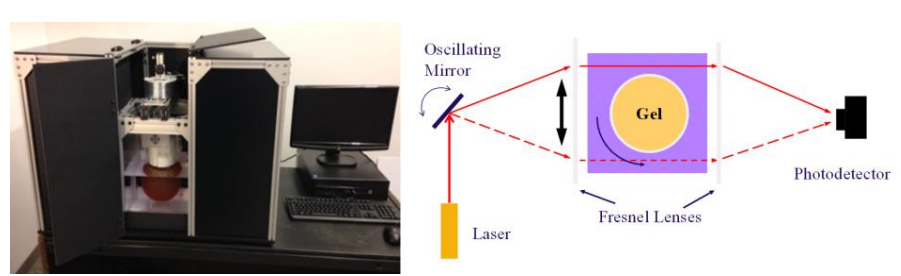
\includegraphics[width=\textwidth]{pictures/LCT_diagram.png}
    \caption{Wygląd oraz schemat tomografu \cite{Mar}}
    \label{fig:LCT}
\end{figure}

Omawiane urządzenie ma przyczynić się do wzrostu bezpieczeństwa i skuteczności radioterapii, jak również przyspieszyć i zoptymalizować pracę samego fizyka medycznego. Z tego powodu, pożądana jest możliwie jak największa automatyzacja działania tomografu. Jednym z aspektów do usamodzielnienia jest diagnostyka działania LCT. Opracowany aparat jest prototypem zbudowanym ręcznie. Trzeba więc w analizie błędów uwzględnić potencjalny czynnik ludzki.

Przy leczeniu wykorzystującym teleradioterapię, niezwykle istotna jest dokładność, jak i precyzja, z jaką deponowana jest dawka promieniowania w guzie nowotworowym oraz jego otoczeniu. W miarę możliwości należy unikać niepotrzebnego narażania tkanek zdrowych oraz narządów krytycznych na uszkodzenia wywołane promieniowaniem. Dlatego też przy symulacjach należy zadbać o możliwie najwierniejsze odzwierciedlenie docelowej operacji, niwelując przy tym błędy mogące wynikać z samego działania urządzenia. W tym celu potrzebna jest dodatkowa aparatura, która umożliwi szybką i sprawną analizę działania samego LCT.

\newpage

Szczególną uwagę trzeba poświęcić silnikowi krokowemu i przymocowanemu do niego zwierciadełku. Kształt zwierciadła (kołowy) pozwala na łatwiejsze zachowanie symetrii. Jednakże, przez potencjalne nieidealne umieszczenie zwierciadła na elemencie obrotowym mogą powstać asymetryczne momenty bezwładności, które będą bezpośrednio wpływać na prędkość obrotową samego elementu (na charakterystyce zmiany położenia objawiłoby się to w postaci niesymetrycznej sinusoidy). Przykładowy silnik krokowy z Amazona przedstawia rysunek 1.2. Kątownik jest przymocowany do silnika, po jednej stronie ma przymocowane zwierciadło, a po drugiej moduł SEN0142 (rozdział 3.3).

\begin{figure}[H]
    \centering
    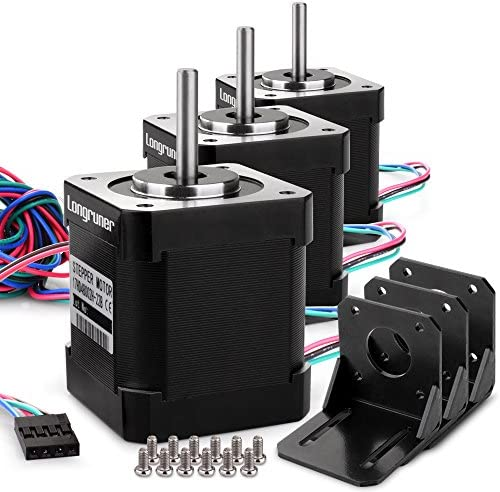
\includegraphics[width=0.6\textwidth]{pictures/silnik.jpg}
    \caption{Przykładowy silnik krokowy}
    \label{fig:silnik}
\end{figure}

Celem pracy jest zaprojektowanie i zbudowanie czujnika wraz z oprogramowaniem, umożliwiającego zautomatyzowany pomiar zmian położenia elementu obrotowego silnika krokowego. Pozwoli to na zaobserwowanie potencjalnych nieprawidłowości w zmianach kątowych poruszającego się zwierciadła, dzięki czemu możliwa będzie szybka reakcja i korekta elementu. Praca ma skupić się na:

\begin{enumerate}
    \item analizie nowych rozwiązań zagadnienia,
    \item zaimplementowaniu wybranego rozwiązania,
    \item testowaniu i udoskonaleniu stworzonego programu.
\end{enumerate}
\chapter{Rozwiązania dostępne na rynku}

\section{Laserowe inklinometry cyfrowe}

Podstawowe cechy:
\begin{itemize}
    \item Cena: $\approx 200$ zł,
    \item niepewność pomiaru: $\pm 0.2^{o}$,
    \item wysoka precyzja,
    \item bezprzewodowe,
    \item przenośne,
    \item zazwyczaj jednoosiowe.
\end{itemize}

Ładowane za pomocą kabla USB (zarówno połączonego do komputera, jak i bezpośrednio do sieci elektrycznej. Mają wbudowaną pamięć, pozwalającą na zapis pomiarów (te mogą być bezwzględne, jak i względne).

Ich wykorzystanie wprowadziłoby ryzyko błędów symulacji LCT wywołanych wiązką laserową z inklinometru.

Przykładowe rozwiązania:
\begin{itemize}
    \item \href{https://www.miniinthebox.com/pl/p/laserowy-katomierz-cyfrowy-inklinometr-linijka-poziomu-lasera-usb-platny-inklinometr-podstawa-magnetyczna-goniometr-magnes-narzedzia-do-pochylania_p8960976.html?currency=PLN&litb_from=paid_adwords_shopping&sku=1_45&country_code=pl&utm_source=google_shopping&utm_medium=cpc&utm_campaign=17688774668&adword_mt=&adword_ct=&adword_kw=&adword_pos=&adword_pl=&adword_net=x&adword_tar=&adw_src_id=3619800739_17688774668__&gclid=Cj0KCQiA5NSdBhDfARIsALzs2EBPmJYEhlH3uvAXeq00x4VJm2TBsisSafEBhxoMUEuFMnTBFwyQr5gaAqf6EALw_wcB}{Laserowy kątomierz cyfrowy - inklinometr}
\end{itemize}

\section{Inklinometry analogowe}

Podstawowe cechy:
\begin{itemize}
    \item Cena: $\approx 2000$ zł,
    \item niepewność pomiaru: $\pm 0.14^{o}$,
    \item zakres poprawnej temperatury: $-40-70^{o}$C
    \item częstotliwość próbkowania: $500$ S/s
    \item wysoka precyzja,
    \item przewodowe,
    \item najczęściej jednoosiowe lub dwuosiowe.
\end{itemize}

Ilość osi, na których czujnik pracuje, jak i precyzja pomiaru są programowalne (drugi parametr jest dodatkowo zależny od zakresu mierzonego kąta). Posiadają również wbudowane filtry antywibracyjne.

Przykładowe rozwiązania:
\begin{itemize}
    \item \href{https://abcelektro.pl/inklinometr-analogowy-seria-is40-8.is40.14121-id-k8-is40-14121-000}{Inklinometr analogowy seria IS40, 8.IS40.14121}
    \item \href{https://sklep.pf-electronic.pl/pl/IN360TC-C2}{CANopen Inklinometr seria IN360TC}
\end{itemize}

\newpage

\section{Inklinometry cyfrowe}

Podstawowe cechy:
\begin{itemize}
    \item Cena: $\approx 250$ zł,
    \item niepewność pomiaru: $\pm 1.15^{o}$
    \item zakres poprawnej temperatury: $-20-125^{o}$C,
    \item przewodowe,
    \item mogą być 3-osiowe,
    \item wrażliwe na wilgoć,
    \item wbudowany interfejs SPI.
\end{itemize}

Są podatne na działanie temperatury - odchylenie jest zaniedbywalne dla temperatury wynoszącej $23^{o}$C \cite{inclino}. Charakterystyki odchyleń w funkcji temperatury prezentuje rys. 2.1.

\begin{figure}[H]
    \subfloat[Oś OX\label{subfig-3:x}]
    {
      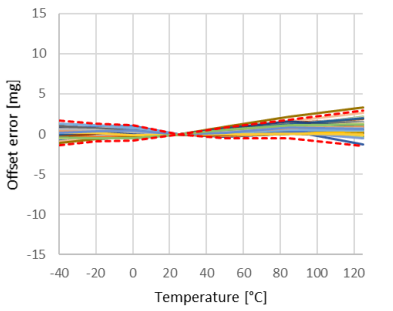
\includegraphics[width=0.45\textwidth]{pictures/tem_x.png}
    }
    \hfill
    \subfloat[Oś OY\label{subfig-4:y}]
    {
      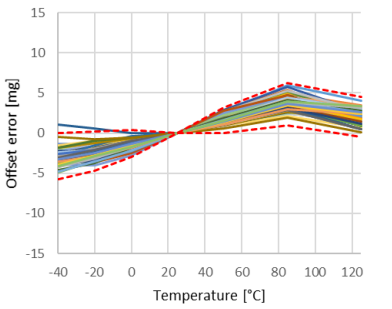
\includegraphics[width=0.45\textwidth]{pictures/tem_y.png}
    }
    \hfill
    \subfloat[Oś OZ\label{subfig-5:z}]
    {
      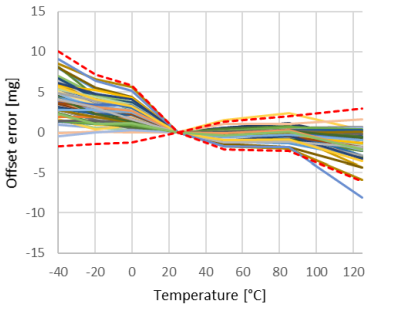
\includegraphics[width=0.45\textwidth]{pictures/tem_z.png}
    }
    \caption{Odchylenia akcelerometru w funkcji temperatury \cite{inclino}}
    \label{fig:inclino_temp}
\end{figure}

Pracuje on na napięciach z zakresu $3.3-3.6$V, możliwe jest więc włączenie go do układu razem z Arduino/Raspberry Pi. Interfejs SPI jest dodatkowym ułatwieniem w komunikacji pomiędzy komponentami.

Przykładowe rozwiązanie:
\begin{itemize}
    \item \href{https://www.mouser.pl/ProductDetail/Murata-Electronics/SCL3300-D01-10?qs=gZXFycFWdAOFydYBLsvu8Q%3D%3D&mgh=1&vip=1&gclid=Cj0KCQiA5NSdBhDfARIsALzs2ECEO9jDFShKG2lA_S2OoNgsOxEbMKKAJx_lWr7MB632r4TBB5kzGLAaAn6aEALw_wcB}{MuRata SCL3300-D01-10}
\end{itemize}
\chapter{ANALIZA ZAGADNIENIA}

\section{Fizyczne zasady działania akcelerometru i żyroskopu}

\subsection{Akcelerometr}

Zadaniem tego podzespołu jest pomiar i analiza przyspieszenia liniowego/kątowego. Wewnątrz urządzenia znajduje się czujnik przyspieszenia, który bada siłę wynikającą ze zmian ruchu. Dzięki dużej wrażliwości na zmianę położenia jest on w stanie określać z dużą precyzją i dokładnością ruch własny, jak i całego akcelerometru. Najczęściej wykorzystuje się 3-osiowe podzespoły (wykonujące pomiar względem osi OX, OY i OZ). Możemy podzielić je na:

\begin{itemize}
    \item piezoelektryczne - mają duże pasmo pomiarowe. Mogą mierzyć drgania o wysokich częstotliwościach i amplitudach. 
    \item piezorezystancyjne - wykorzystywane do pomiarów wibracji. Stosowane powszechnie w przemyśle.
    \item pojemnościowe MEMS - najmniejsze i najtańsze. Zostały zastosowane w opracowywanym prototypie.
\end{itemize}

W przypadku akcelerometrów MEMS pomiar polega na badaniu zmian pojemności pomiędzy ruchomą masą a nieruchomymi okładkami kondensatora. Podczas ruchu z przyspieszeniem zmienia się pojemność, którą następnie można przekonwertować na potrzebną wartość. Wadą tych elementów (korygowaną stopniowo przez producenta) jest stosunkowo mała czułość i podatność na szumy. Rysunek 3.1 przedstawia przykładową charakterystykę niezamocowanego modułu wprawionego w ruch symulujący ten z tomografu.

\begin{figure}[H]
    \centering
    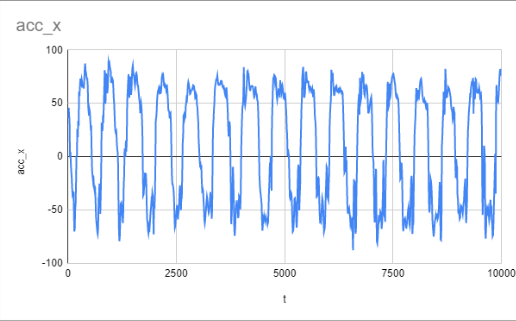
\includegraphics[width=0.9\textwidth]{pictures/raw.png}
    \caption{Przykładowa charakterystyka z akcelerometru A [ref] = f(t [ms])}
    \label{fig:raw}
\end{figure}

\newpage

Dla wartości względem osi OX i OY przesyłanych przez urządzenie stosuje się przekształcenia, umożliwiające otrzymanie odpowiednio: kąta pochylenia (ang. pitch) $\theta$, jak i przechylania (ang. roll) $\phi$ :

\begin{equation}
    \theta = \arctan \Bigg( \frac{A_{x}}{\sqrt{A_{y}^{2} + A_{z}^{2}}} \Bigg)
\end{equation}
\begin{equation}
    \phi = \arctan \Bigg( \frac{A_{y}}{\sqrt{A_{x}^{2} + A_{z}^{2}}} \Bigg)
\end{equation}

Powyższe wzory wynikają bezpośrednio z twierdzenia Pitagorasa zastosowanego w przestrzeni trójwymiarowej ($A$ - wektor przyspieszenia).

\subsection{Żyroskop}

Żyroskopy to urządzenia służące do analizy, jak i utrzymywania orientacji przestrzennej. Można je podzielić na kierunkowe, prędkościowe i elektroniczne. Służą do mierzenia prędkości obrotowej obiektu. Drgania elementu zostają wymuszone dzięki efektowi piezoelektrycznemu, natomiast pomiar wykorzystuje siłę Coriolisa (złożenie dwóch ruchów pewnej masy, z czego jeden jest ruchem  obrotowym) \cite{filtr}.

By otrzymać zmianę kąta, otrzymane dane należy scałkować po czasie, co prezentują poniższe równania \cite{filtr}:

\begin{equation}
    \theta(t_{i}) = \theta(0) + \sum^{i}_{j=1} \omega_{X}(t_{j})(t_{j} - t_{j-1})
\end{equation}
\begin{equation}
    \phi(t_{i}) = \phi(0) + \sum^{i}_{j=1} \omega_{Y}(t_{j})(t_{j} - t_{j-1}),
\end{equation}
\begin{equation}
    \psi(t_{i}) = \psi(0) + \sum^{i}_{j=1} \omega_{Z}(t_{j})(t_{j} - t_{j-1}),
\end{equation}

\noindent gdzie: $\theta$ - kąt przechylania (pitch), $\phi$ - kąt pochylania (roll), $\psi$ - kąt skręcenia (yaw), $\omega$ - prędkość obrotowa i jej odpowiednie składowe względem danej osi, $t$ - czas.

\subsection{Filtr Kalmana}

Otrzymywane pomiary podatne są na zakłócenia: akcelerometr jest wyczulony na drgania otoczenia, natomiast żyroskop jest podatny na zjawisko dryfu. Dodatkowo, ze względu na dane z dwóch czujników, należy dokonać ich złożenia. Do tego celu stosuje się między innymi  filtr Kalmana, który dokonuje iteracyjnej estymacji procesu w układzie ze sprzężeniem zwrotnym \cite{filtr}. Możemy wyznaczyć dwie fazy działania filtru: fazę predykcyjną i fazę korekcji.

W praktyce zostanie wykorzystany cyfrowy filtr Kalmana realizujący algorytm rekurencyjny. Bazując na \cite{kal}, model estymacji możemy przedstawić jako: liniowe równanie stanu i liniowe równanie obserwacji (odpowiednio (3.6) i (3.7)).

\newpage

\begin{equation}
    x(t+1) = A(t)x(t) + B(t)v(t)
\end{equation}
\begin{equation}
    y(t) = C(t)x(t) + w(t)
\end{equation}

\noindent gdzie: $t$ - wartości dyskretne na osi czasu, $x(t)$ - wektor stanu, $y(t)$ - wektor obserwacji, $v(t)$ - biały szum procesowy o zerowej wartości średniej, $w(t)$ - biały szum obserwacji o zerowej wartości średniej, $A(t)$ - macierz systemowa, $B(t)$ - macierz wejścia, $C(t)$ - macierz wyjścia.

Następnie w fazie korekcji algorytm wykorzystuje pomiary do aktualizacji i poprawy estymacji. W publikacji \cite{kal} została przedstawiona dalsza metodologia działania tych filtrów.

\section{Płytka Arduino Uno}

Arduino to projekt rozpoczęty w roku 2005, opierający się na licencji typu \textit{open hardware}. Przeznaczony on jest dla mikrokontrolerów zamontowanych na obwodzie drukowanym z wbudowanymi układami wejścia/wyjścia (I/O) oraz standaryzowanym językiem programowania. Ostatni bazuje na C++, a wykorzystując wtyczkę PlatformIO możliwe jest kompletne posługiwanie się tym językiem.

W projekcie zostanie wykorzystany model Arduino Uno. Został on wybrany na podstawie dostępnych funkcjonalności, przy akceptowalnej cenie produktu. Opracowywane oprogramowanie nie będzie zapisywać danych na płytce, lecz będą one przesyłane i przechowywane w aplikacji okienkowej. 

\begin{figure}[H]
    \centering
    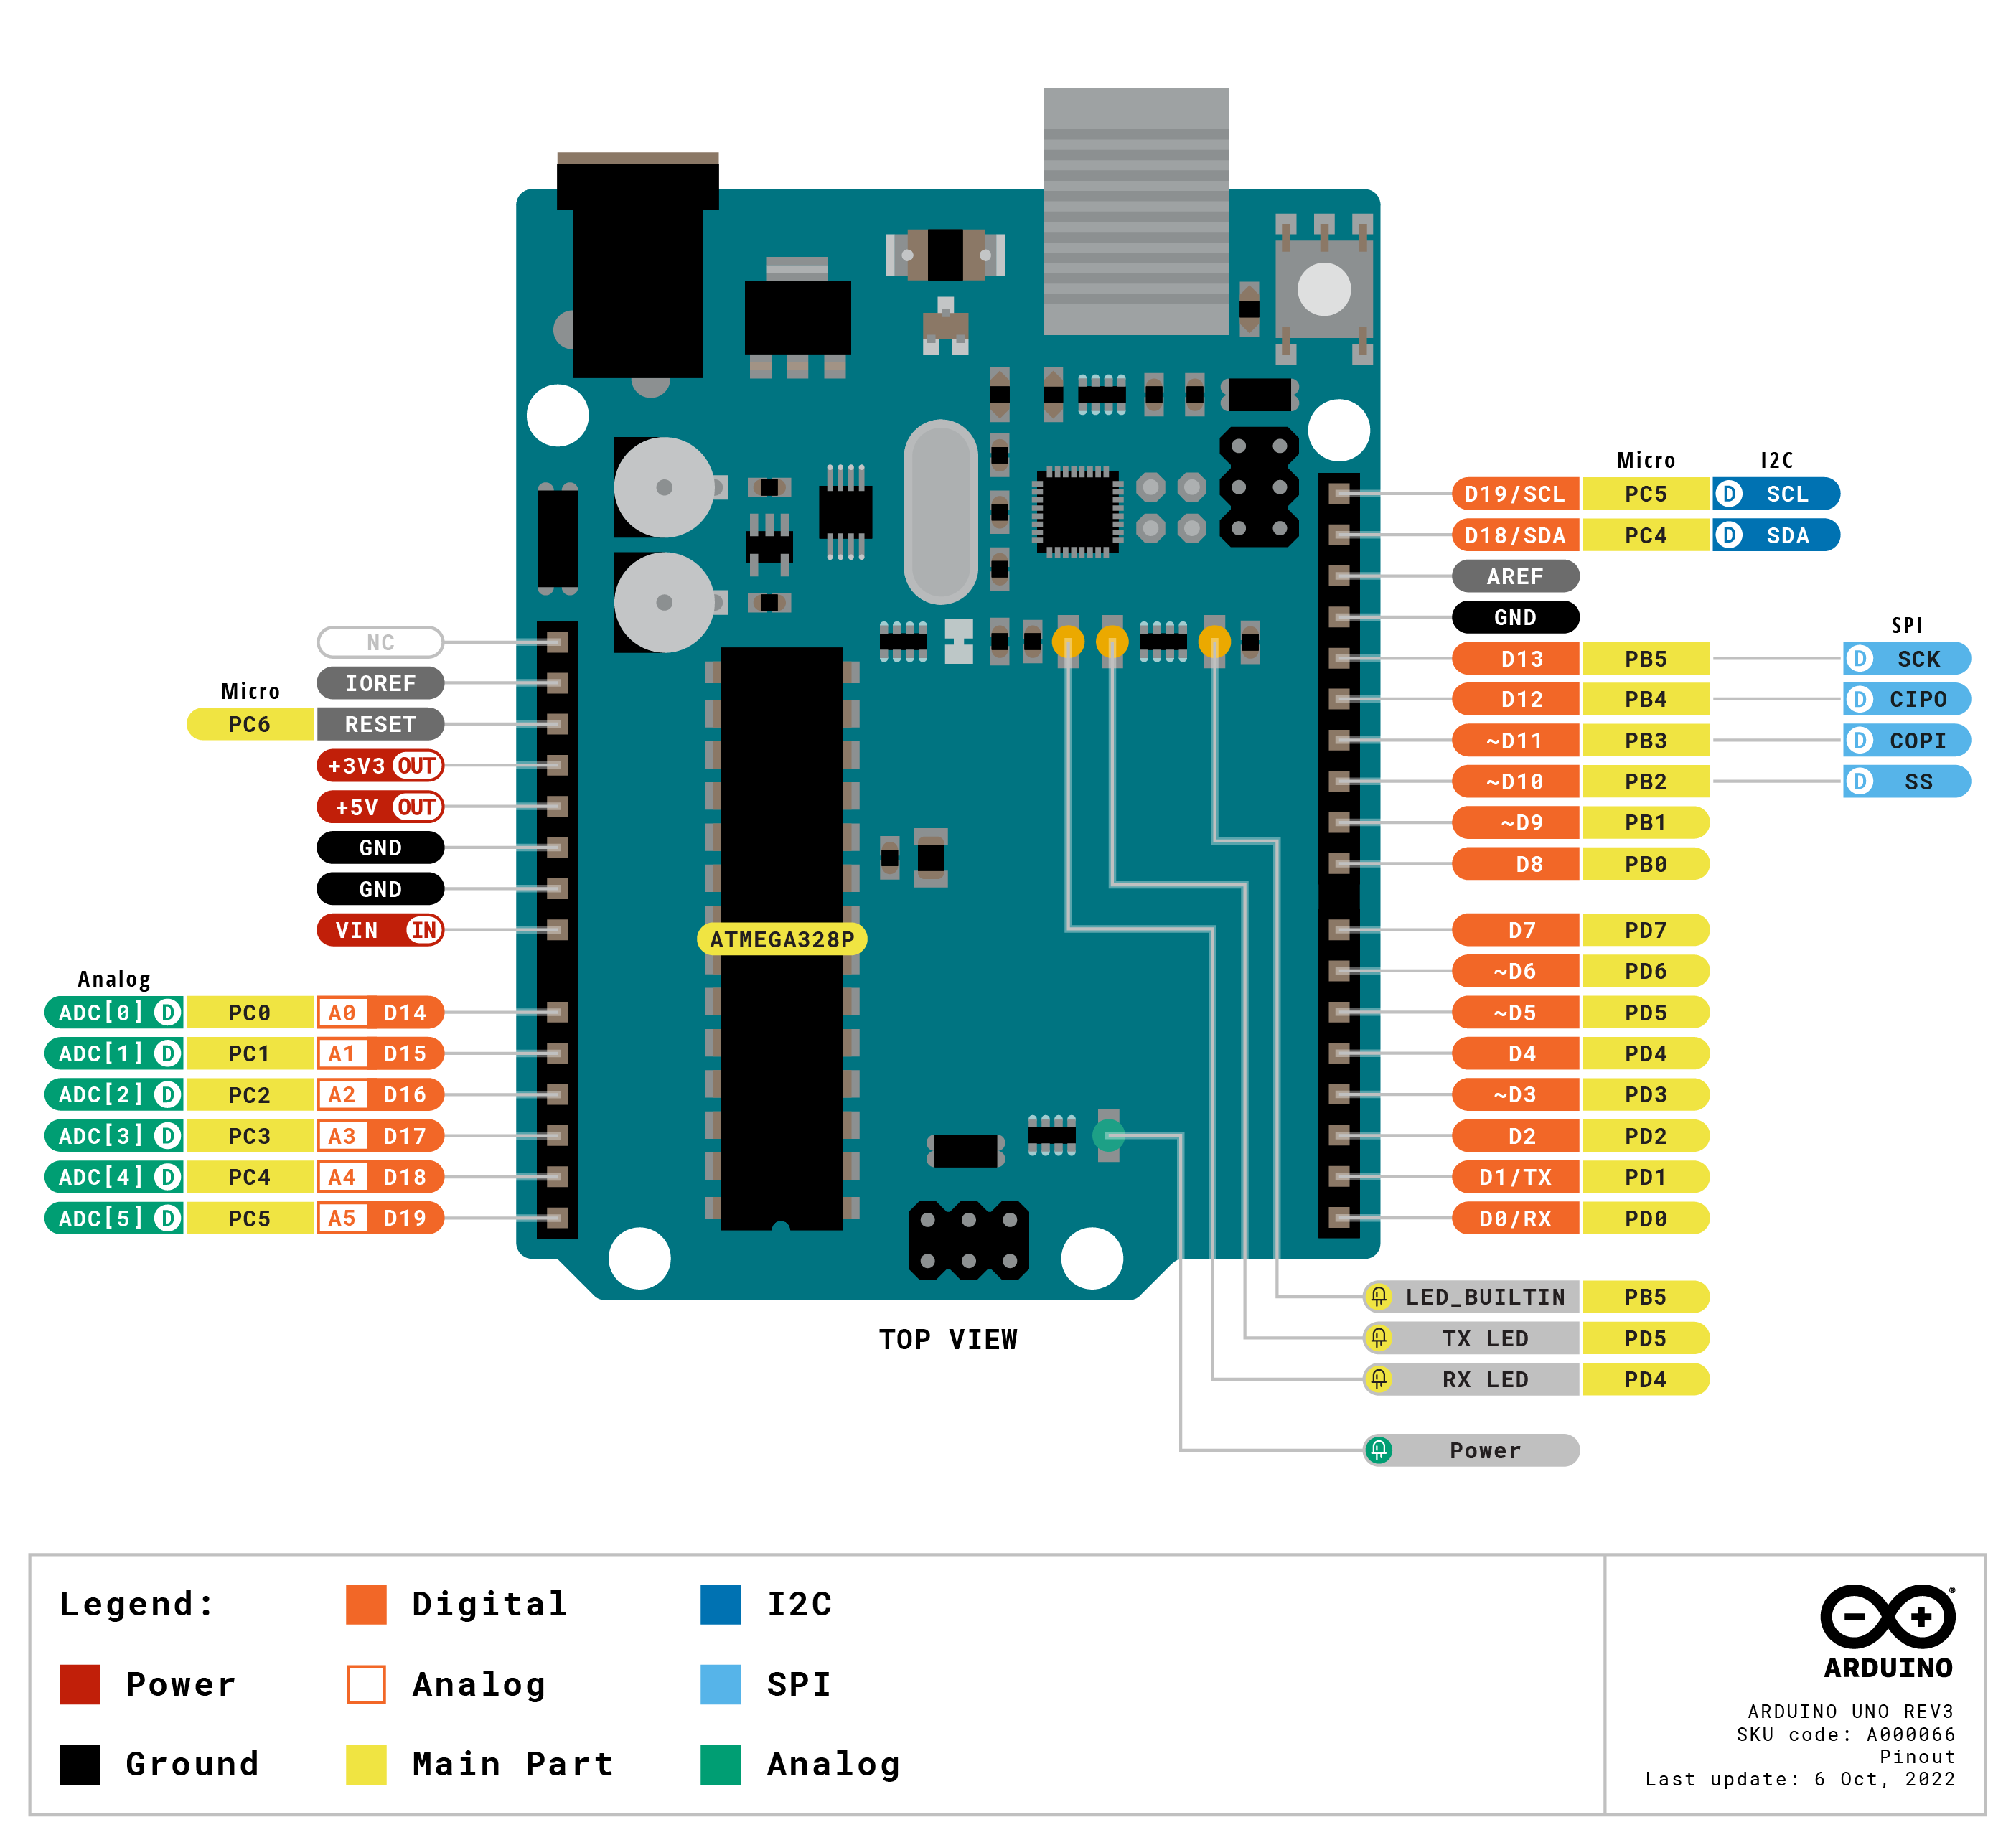
\includegraphics[width=0.9\textwidth]{pictures/uno.png}
    \caption{Schemat Arduino Uno \cite{Ardocs}}
    \label{fig:ard_vague}
\end{figure}

Sama płytka składa się z 8-bitowego mikrokontrolera Atmel AVR (konkretnie ATmega328P), ma wbudowane 32KB pamięci flash, 2KB SRAM, 1KB EEPROM. Posiada interfejsy: I2C, SPI, UART i USB (jest programowana przez adapter \textit{USB to serial}). Działa na napięciach wejścia 7-12V oraz wartościach napięć operacyjnych 3.3V i 5V. Płytka posiada 20 pinów cyfrowych oraz 6 analogowych i typu PWM. Rys. 3.2 przedstawia umiejscowienie powyższych funkcji na płytce drukowanej.

Oficjalnym środowiskiem do programowania omawianych płytek jest Arduino IDE. Aczkolwiek, ze względu na stosunkowo ograniczone możliwości w pracy zostanie wykorzystane JetBrains CLion wraz z wtyczką PlatformIO. Oprogramowanie to posiada znacznie większe możliwości, jako że producent specjalizuje się w narzędziach programistycznych, zarówno na licencjach płatnych, jak i tych typu \textit{open source}.

\section{Moduł DFRobot SEN0142 (MPU-6050) - dodatek do Arduino}

MPU-6050 opracowane przez firmę InvenSense są powszechnie używane w modułach określających położenie w przestrzeni, jak i prędkością obrotową. Charakteryzują się one małym poborem mocy oraz wysoką wydajnością. Podzespoły te zawierają w sobie dwa analogowe czujniki: akcelerometr i żyroskop. Oba pozwalają na pomiar zmiany kąta, jednak na odmiennej zasadzie. Sam moduł posiada wbudowany cyfrowy procesor ruchu, jak i 16-bitowy przetwornik analogowo-cyfrowy (ADC). Wykorzystując magistralę I2C wraz z wbudowanymi rezystorami, możliwe jest (poprzez komunikację szeregową) uzyskanie zestawów danych przy bezpośrednim połączeniu układu z Arduino.

Na rynku jest dostępnych wiele podzespołów z wbudowanym układem MPU-6050. Moduł od firmy DFRobot został wytypowany ze względu na posiadanie funkcji wystarczających do spełnienia założeń doświadczenia przy akceptowalnej cenie. Dodatkowym atutem jest rozmiar czujnika, który całkowicie mieści się na elemencie obrotowym silnika krokowego. Rys. 3.3 prezentuje zespolenie MPU-6050 z całym modułem SEN0142.

\begin{figure}[H]
    \centering
    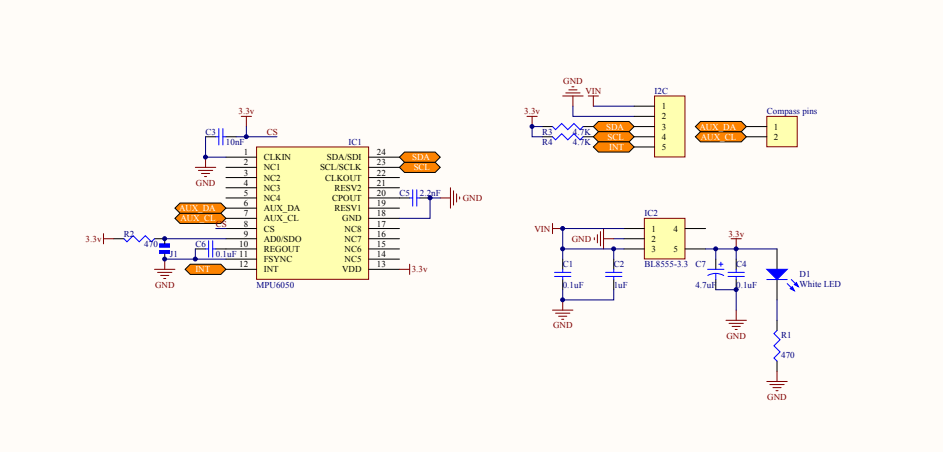
\includegraphics[width=\textwidth]{pictures/short_schema.png}    
    \caption{Schemat modułu DFRobot SEN0142 \cite{shop}}
    \label{fig:DFRobot_scheme}
\end{figure}

\newpage

\subsection*{Specyfikacja na podstawie \cite{dfr}}

\begin{enumerate}
    \item \textbf{Akcelerometr}
    \begin{itemize}
        \item Trzyosiowy, z cyfrowym wyjściem, programowalny w zakresie przeciążeń: $\pm 2\;g$, $\pm 4\;g$, $\pm 8\;g$ i $\pm 16\;g$
        \item Posiada zintegrowane, 16-bitowe przetworniki ADC, pozwalające na próbkowanie sygnałów bez stosowania multiplekserów
        \item Natężenie prądu roboczego: $500 \mu A$
        \item Natężenie prądu przy niskim poborze mocy: $10\; \mu A$ dla $1.25\; Hz$, $20\; \mu A$ dla $5\; Hz$, $60\; \mu A$ dla $20\; Hz$, $110\; \mu A$ dla $40\; Hz$
    \end{itemize}
    \item \textbf{Żyroskop}
    \begin{itemize}
        \item Trzyosiowy, z cyfrowym wyjściem, programowalny w przedziale prędkości kątowych: $\pm 250$, $\pm 500$,  $\pm 1000$ i  $\pm 2000 ^{o}/s$
        \item Wbudowane 16-bitowe ADC
        \item Poprawiona wydajność (względem poprzednich modeli) szumów przy niskich częstotliwościach
        \item Programowalny cyfrowy filtr dolnoprzepustowy
        \item Natężenie prądu roboczego: $3.6\; mA$
        \item Natężenie prądu spoczynkowego: $5\; \mu A$
    \end{itemize}
\end{enumerate}



\section{Budowa i założenia działania czujnika}

\subsection{Budowa}

Czujnik składa się z dwóch elementów: płytki Arduino oraz modułu DFRobot SEN0142 połączonych czterema przewodami, jak pokazano na Rys. 3.4.

\begin{figure}[H]
    \centering
    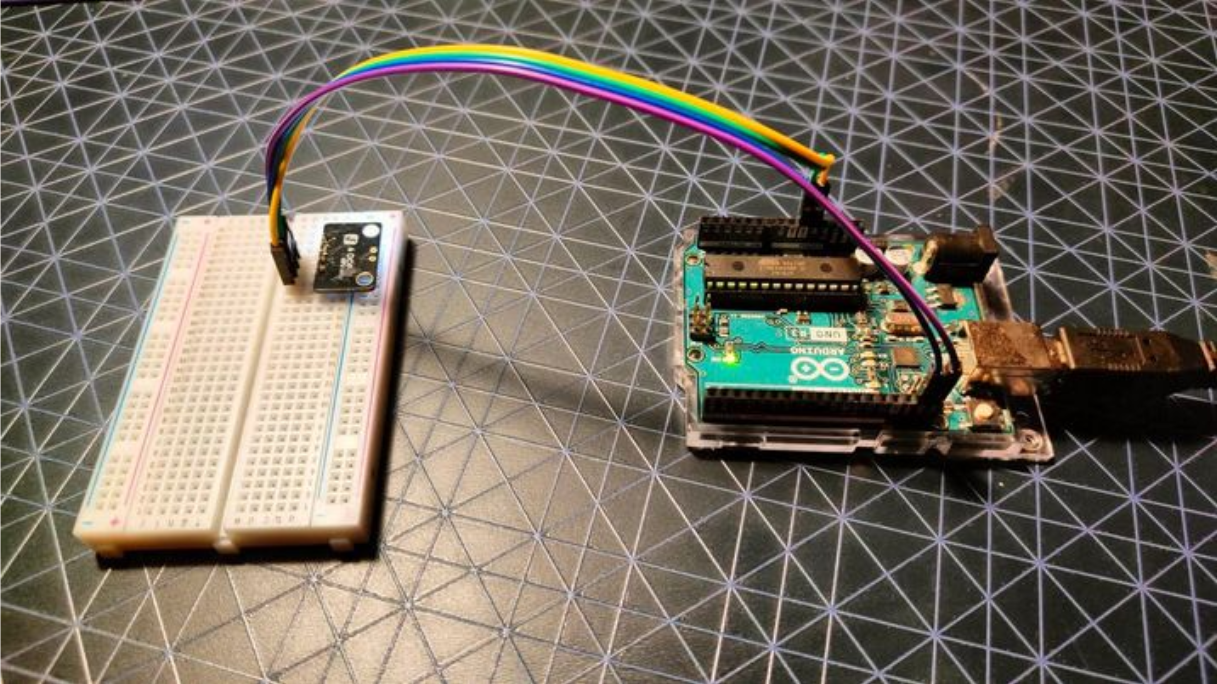
\includegraphics[width=\textwidth]{pictures/prototype.png}
    \caption{Pierwszy prototyp urządzenia}
    \label{sketch}
\end{figure}

Moduł SEN0142 zasilany jest stałym napięciem 5V. SDA i SCL są pinami magistrali I2C odpowiadającymi odpowiednio za: linię danych (serial data) oraz linię zegara taktującego tranmisję (serial clock).

\subsection{Magistrala I2C i port szeregowy}
Komunikacja pomiędzy Arduino a modułem SEN0142 przebiega poprzez szynę I2C. Jak przedstawiono w \cite{forbot}, obie linie magistrali są dwukierunkowe, rezystor podciągający podłącza je do dodatniego napięcia. Gdy nie ma transmisji, to zarówno na SDA i SCL znajduje się stan wysoki. Standardowo dane są przesyłane z prędkością 100 kb/s, lub 400 kb/s. 

Każdy układ podłączony do magistrali ma przypisany adres i może być zarówno odbiornikiem jak i nadajnikiem. Dzielimy je na tzw.: master i slave. Pierwszy inicjuje transmisję i generuje sygnał zegarowy. Drugim natomiast jest każdy zaadresowany układ. Rola mistrza najczęściej jest przypisana mikrokontrolerom, podobnie w przypadku tego projektu: płytce Arduino. 

Napięcia poziomów logicznych nie są zdefiniowane, ale zależą od napięcia zasilającego $V_{dd}$. Jeden impuls zegarowy przypada na każdy przesłany bit. Dla wysokiego poziomu zegara wymagana jest stabilność danych na lilii SDA. Stan może się zmieniać dla niskiego zegara.

\begin{figure}[H]
    \centering
    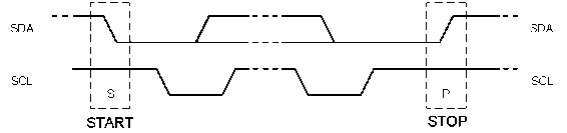
\includegraphics[width=0.95\textwidth]{pictures/ss.png}
    \caption{Bity start i stop \cite{forbot}}
    \label{fig:ss}
\end{figure}

Gdy na SCL panuje stan $1$ a na SDA następuje zmiana:

\begin{itemize}
    \item $1 \rightarrow 0$, następuje bit START,
    \item $0 \rightarrow 1$, następuje bit STOP.
\end{itemize}

Obie sytuacje są generowane przez układ master. Po bicie START szyna jest zajęta, a po STOP się zwalnia.

Komunikacja pomiędzy Arduino a komputerem stacjonarnym odbywa się poprzez UART, kabel USB i port szeregowy.

\begin{figure}[H]
    \centering
    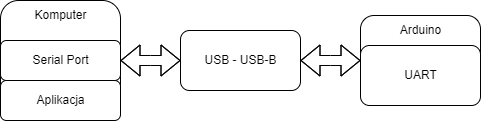
\includegraphics[width=0.8\textwidth]{pictures/serialPort.png}
    \caption{Schemat komunikacji}
    \label{fig:sp}
\end{figure}

Port szeregowy jest typem portu komputerowego, gdzie przekazane dane mają formę ciągu bitów. Jest zdolny do tłumaczenia bitów na bajty i odwrotnie. Jako, że komputer posiada kilka takich portów, należy upewnić się, który z nich przypada na Arduino. Otwierając komunikację istnieje również opcja między innymi: wyboru prędkości połączenia.
\chapter{ANALIZA OPRACOWANEGO OPROGRAMOWANIA}

Opracowane oprogramowanie działa na zasadzie akcja-reakcja. W zależności od nastaw w aplikacji, ta wysyła odpowiedni ciąg znakowy do Arduino, które na tej podstawie wykonuje odpowiedni pomiar. Otrzymywane dane są na bieżąco przesyłane z powrotem do aplikacji, gdzie ta wyświetla je w oknie tekstowym. Po otrzymaniu wszystkich wyników, program może:

\begin{itemize}
    \item przekonwertować dane na odpowiedni format, umożliwiając tym samym wizualizację otrzymanych danych,
    \item zapisać dane do pliku tekstowego w przygotowanym folderze, nadając mu nazwę złożoną z daty i godziny pomiaru.
\end{itemize}

Przesyłanie danych pomiarowych bezpośrednio do komputera było konieczne ze względu na małą pamięć płytki Arduino. Wiąże się to jednak z pewnym utrudnieniem, wynikającym bezpośrednio z działania portu szeregowego. Mianowicie, komenda przesyłania danych \lstinline{Serial.print()} jest powolna. Z tego powodu, pomimo działania zegara magistrali I2C nawet na częstotliwości $400$ kHz, w rzeczywistości osiągalna jest częstotliwość jedynie $100$ Hz. Powinno jednak być to wystarczające do analizy potencjalnych różnic w momentach bezwładności poruszającego się zwierciadła, jak i potencjalnych odchyleń od położenia referencyjnego.

\section{Skrypt do Arduino}

Każdy skrypt Arduino do poprawnego działania wymaga dwóch funkcji: \lstinline{void setup()} oraz \lstinline{void loop()}. Pierwsza służy do konfiguracji parametrów, wykonywana jest tylko przy uruchomieniu płytki, druga natomiast jest nieskończoną pętlą wykonującą się tak długo, dopóki Arduino jest podłączone do zasilania (czy to przez USB-B, czy bezpośrednio do źródła (np. bateria 9V).

Przy definicjach funkcji został zastosowany dodatkowy człon \lstinline{__attribute__((unused))}. Jest on jedynie informacją dla środowiska, by to nie wyświetlało błędu o niewykorzystaniu owych funkcji (nie są one w żadnym momencie wywoływane). Omawiane funkcje prezentują się następująco:

\lstinputlisting[caption=Funkcja loop(), language=c++, firstline=56, lastline=68]{listings/main.cpp}

\newpage

\lstinputlisting[caption=Funkcja setup(), language=c++, firstline=41, lastline=50]{listings/main.cpp}

Listing 4.1 prezentuje ciało kluczowej funkcji - właśnie ona rozporządza wywoływaniem odpowiednich funkcji w zależności od odczytanego znaku. Wartość $10$ odpowiada co ile milisekund jest próbkowany sygnał z czujnika, natomiast $10000$ to czas pełnego pomiaru, również w milisekundach.

Drugi listing natomiast prezentuje ustawienie parametru częstotliwości zegara, na którym będzie operować szyna I2C ($400$ kHz). Zostaje również ustawiona prędkość portu szeregowego.

Prócz opisanych funkcji, skrypt posiada jeszcze trzy dodatkowe, kluczowe do wykonania i obróbki pomiarów z postaci surowej do wartości docelowych.

Funkcja badająca położenie czujnika (w stopniach, względem wektora siły grawitacyjnej) opiera się na złożeniu pomiarów z akceleratora i żyroskopu przy pomocy filtra Kalmana (zaimplementowany z biblioteki).

\lstinputlisting[caption=Funkcja filtered\_angles(), language=c++, firstline=86, lastline=110]{listings/main.cpp}

Definicje filtrów muszą być umieszczone poza pętlą, w przeciwnym wypadku byłyby one z każdą kolejną iteracją resetowane, w efekcie czego wartości byłyby złożeniem zmiany kątów, a nie położenia. Otrzymane dane z akcelerometru zostają przeliczone na kąty za pomocą wzorów (3.5) i (3.6). Wyniki po fuzji sensorycznej IMU zostają przesłane na komputer.

\lstinputlisting[caption=Funkcja get\_gyr(), language=c++, firstline=112, lastline=135]{listings/main.cpp}

Listing 4.4 jest w rzeczywistości implementacją wzorów (3.3) i (3.4) z uwzględnieniem czasu trwania pomiaru. Dodatkowo, linie 19-20 są odpowiedzialne za włączanie/wyłączanie diody wraz z wykonywaniem kolejnych pomiarów. Funkcja \lstinline{show()} służy do przesyłania wyników do komputera w sformatowanej formie, ułatwiając potem aplikacji rozdzielanie danych do odpowiednich tablic.

\section{Aplikacja}

\subsection{Wygląd i funkcjonalności}

Okno aplikacji prezentuje się następująco:

\begin{figure}[H]
    \subfloat[Okno bez płytki\label{subfig-1:wo}]
    {
      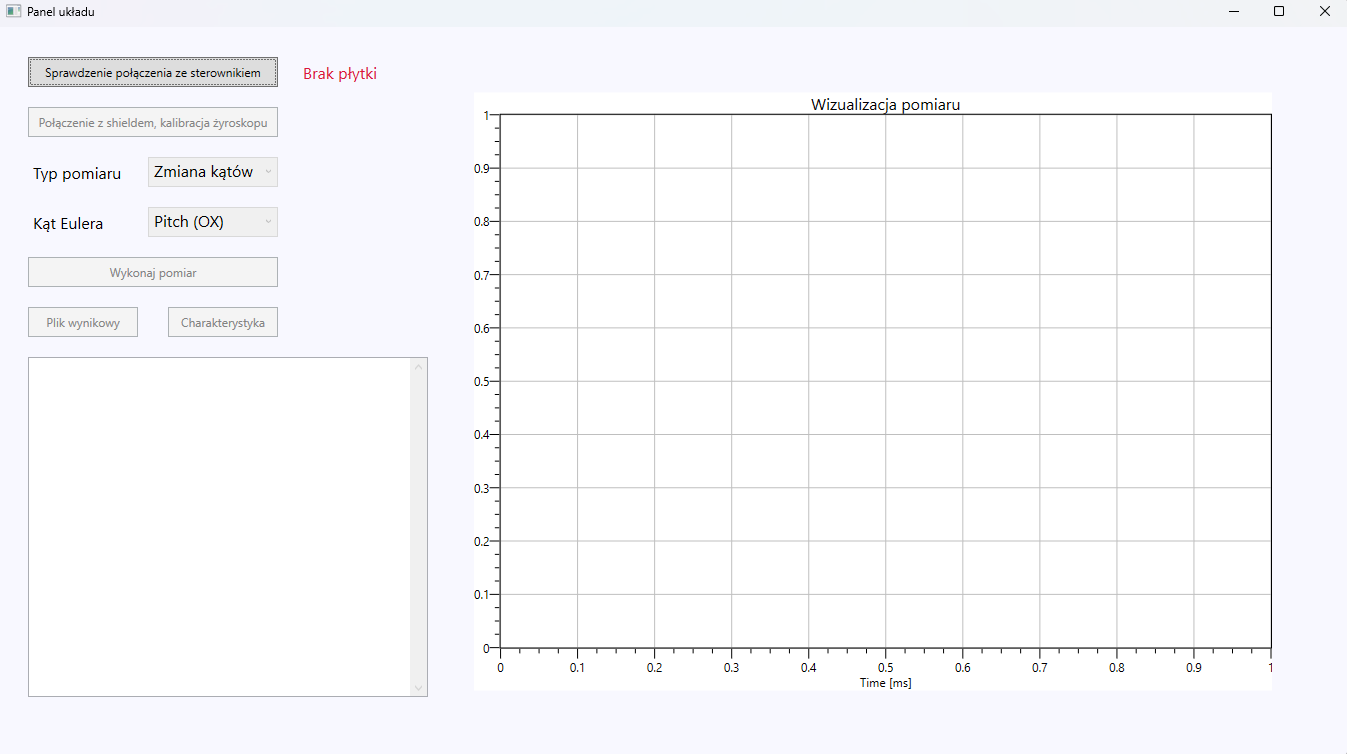
\includegraphics[width=0.48\textwidth]{pictures/app_wo.png}
    }
    \hfill
    \subfloat[Okno z płytką\label{subfig-2:w}]
    {
      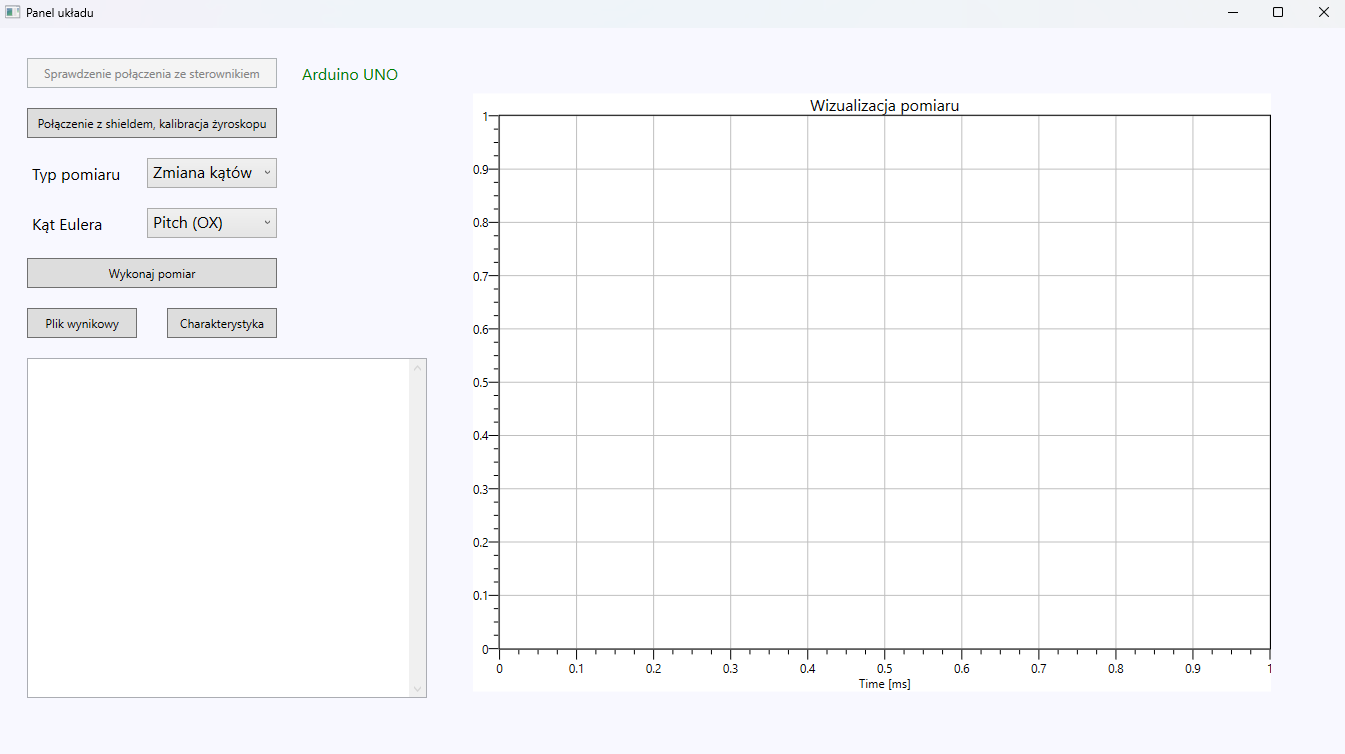
\includegraphics[width=0.48\textwidth]{pictures/app_w.png}
    }
    \caption{Okno aplikacji}
    \label{fig:app}
\end{figure}

Aplikacja pozwala na pomiar:

\begin{itemize}
    \item położenia względem wektora przyspieszenia ziemskiego względem osi OX i OY (charakterystyka przedstawia jednocześnie dane przed i po przefiltrowaniu),
    \item zmian jednego z kątów RPY (wybranego),
    \item pomiar szumów (ponownie z filtrem i bez) - położenie dla nieruchomego czujnika.
\end{itemize}

Okno aplikacji po wykonaniu pomiaru prezentuje następujące informacje (Rys. 4.2): nastawy wyboru (położenie i pitch), wartości pomiarowe w oknie tekstowym oraz wykres zależności wybranego kąta od czasu.

\begin{figure}[H]
    \centering
    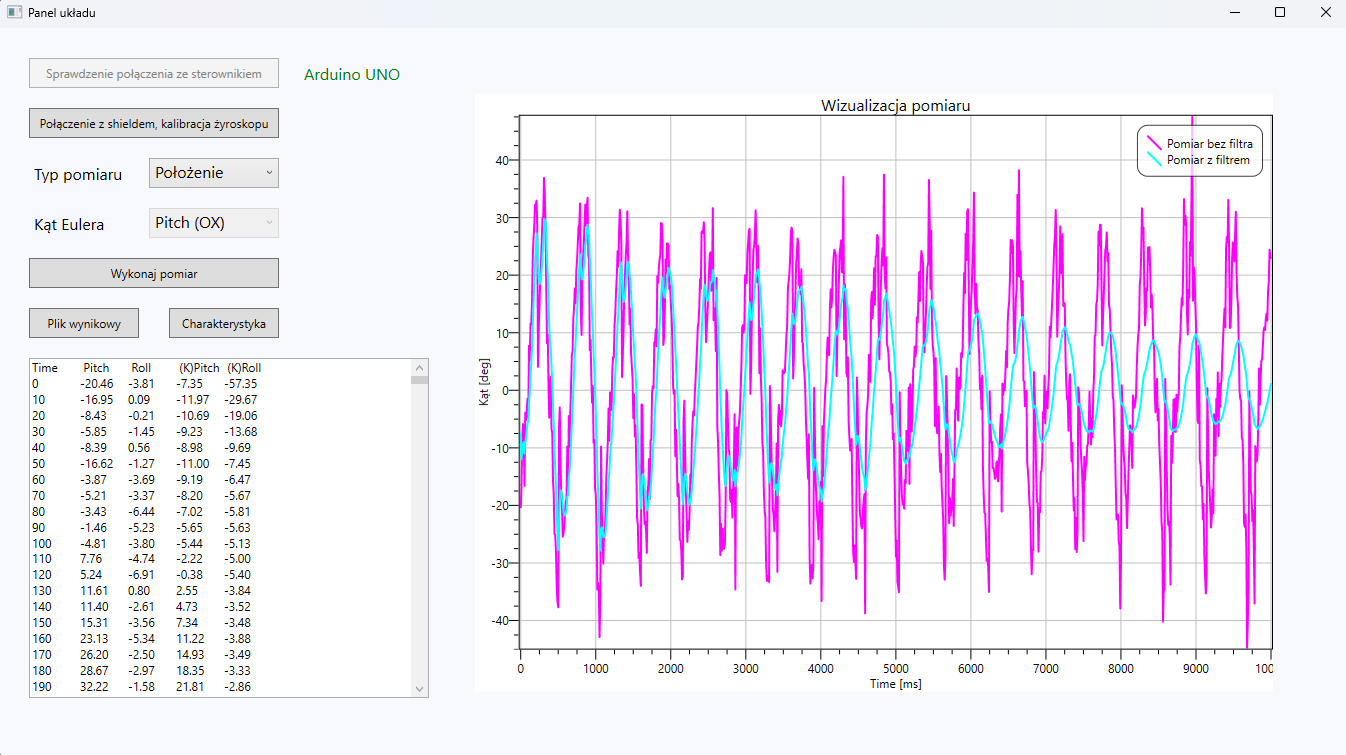
\includegraphics[width=\textwidth]{pictures/example.png}
    \caption{Przykład działania aplikacji}
    \label{fig:my_label}
\end{figure}

\subsection{Klasa aplikacji}

\lstinputlisting[caption=Metoda BtnStart\_OnClick(), language=csh, firstline=99, lastline=120]{listings/MainWindow.xaml.cs}

Listing 4.5 prezentuje główną metodę programu (odpowiadającą za obsługę przycisku \emph{Wykonaj pomiar}). Wyglądem przypomina funkcję \lstinline{void loop()}, z tą różnicą, że ta wysyła informację. Wariant dla szumu i położenia wysyła tę samą informację do płytki Arduino, ten pierwszy jednak dodatkowo zmienia jeszcze tytuł wykresu. Jako, że aplikacja w czasie rzeczywistym wyświetla pomiary w oknie tekstowym, należało wprowadzić wielowątkowość (linia 21), która umożliwia oprogramowaniu śledzenie zmian w zmiennej odbierającej dane (na bazie \cite{csh}).

Jednak zanim możliwe będzie wykonanie pomiarów, program musi upewnić się, że płytka Arduino jest dostępna. Służy do tego metoda \lstinline{BtnCheck_OnClick()}.

\lstinputlisting[caption=Metoda BtnCheck\_OnClick(), language=csh, firstline=71, lastline=93]{listings/MainWindow.xaml.cs}

Powyższy fragment kodu próbuje uruchomić połączenie szeregowe. Jeśli jest to wykonalne, kontakt zostanie nawiązany (o czym program poinformuje) i odblokowane zostaną wszystkie nastawy. W przeciwnym wypadku zostanie wystosowany komunikat o braku płytki (Rys. 4.1).

Ze względu na specyfikę kompilatora języka C\# należało opracować metodę do modyfikacji danych (listing 4.7), ponieważ ten wymusza separator dziesiętny w zależności od ustawień regionalnych systemu operacyjnego. Okazało się to o tyle problematyczne, że dane generowane przez moduł SEN0142 część ułamkową miały zapisaną po kropce, gdy w Polsce oficjalnie jest to przecinek. Metoda (dla pomiarów z filtrem) dodatkowo pomija pomiary z pierwszych $200$ ms, ze względu na wartości z filtra, które są obarczone błędem grubym.

\newpage

\lstinputlisting[caption=Metoda ModifyData(), language=csh, firstline=225, lastline=242]{listings/MainWindow.xaml.cs}

Największą i najbardziej skomplikowaną metodą jest \lstinline{BtnShow_OnClick()}. Odpowiada on w głównej mierze za rysowanie wykresów. Na poniższych listingach zostały zaprezentowane jedynie najważniejsze fragmenty kodu - ze względu na bardzo dużą ilość warunków logicznych, gdzie na każdą wariację przypadają podobne akcje, co najwyżej z innymi parametrami. Pokazano również fragmenty o unikalnym działaniu.

\lstinputlisting[caption=BtnShow\_OnClick - rozdzielanie danych), language=csh, firstline=139, lastline=140]{listings/MainWindow.xaml.cs}

Listing 4.8 prezentuje podział danych pobranych z okna tekstowego aplikacji za pomocą systemu zapytań kwerend LINQ. Na podstawie konkretnej sekwencji ucieczki (\lstinline{\n} lub \lstinline{\t}) dane są odpowiednio podzielone na dwuwymiarową tablicę.

\lstinputlisting[caption=BtnShow\_OnClick - kreślenie charakterystyki, language=csh, linerange={154-159,164-164,173-176}]{listings/MainWindow.xaml.cs}

Listing 4.9 prezentuje kolejne polecenia, które trzeba wykonać, by otrzymać charakterystykę. Wymagane jest każdorazowe wyczyszczenie siatki wykresu w celu zlikwidowania poprzednich wykresów.

\lstinputlisting[caption=BtnShow\_OnClick - zapobieganie złemu kreśleniu, language=csh, firstline=191, lastline=193]{listings/MainWindow.xaml.cs}

Jako, że położenie mierzone jest względem osi $OX$ lub $OY$, należy zabezpieczyć oprogramowanie przed potencjalną próbą wykonania analogicznej operacji dla osi $OZ$. Powyższy listing sprawia, że w przypadku takiej próby, program wyświetli komunikat z ostrzeżeniem.

Ostatnia metoda, którą użytkownik może wywołać za pomocą przycisku, jest zapisanie pomiarów do pliku tekstowego (.txt). Funkcja jednak nie tworzy katalogu, zakłada że taki już istnieje.

\lstinputlisting[caption=Metoda BtnFile\_OnClick(), language=csh, firstline=125, lastline=131]{listings/MainWindow.xaml.cs}

\section{Pomiar szumów}

W celu oceny wykonano dwa pomiary szumów - dla czujnika leżącego i stojącego. Otrzymano następujące charakterystyki:

\begin{figure}[H]
    \subfloat[Szum dla $\theta$\label{subfig-3:theta_sit}]
    {
      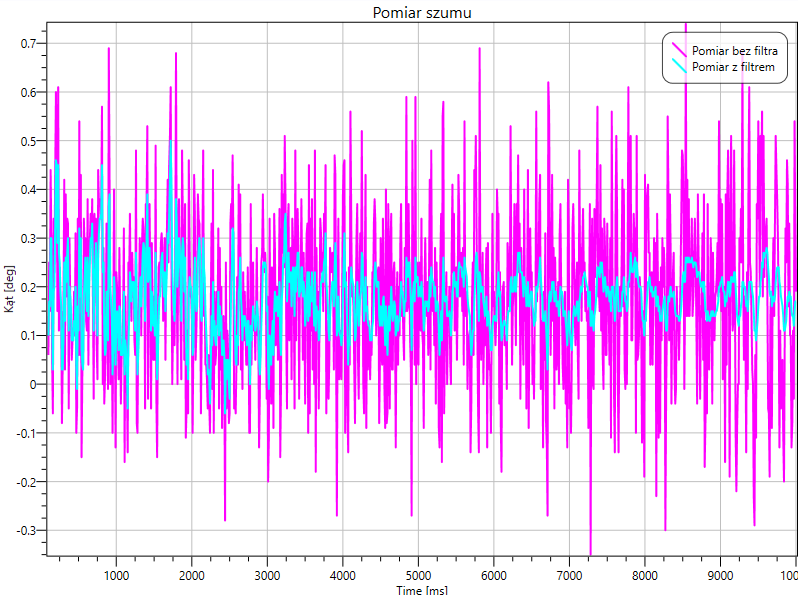
\includegraphics[width=0.48\textwidth]{pictures/theta_sit.png}
    }
    \hfill
    \subfloat[Szum dla $\phi$\label{subfig-4:phi_sit}]
    {
      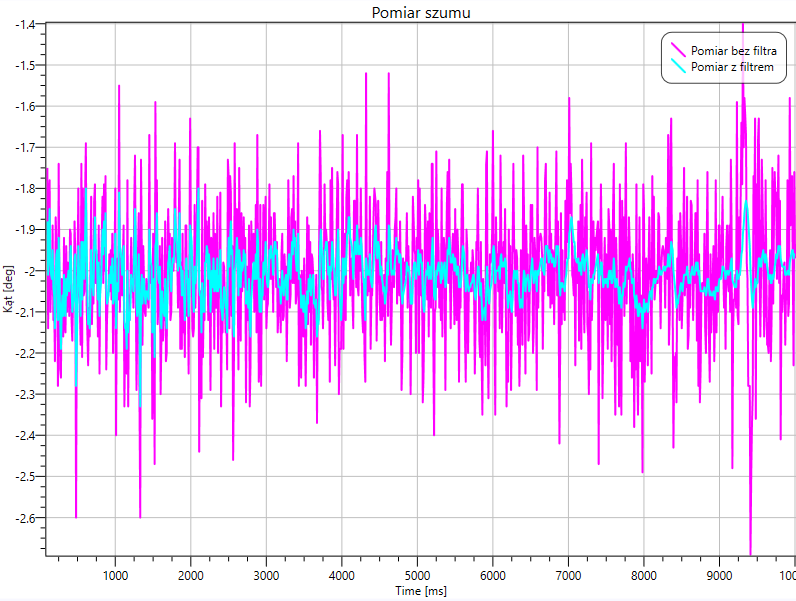
\includegraphics[width=0.48\textwidth]{pictures/phi_sit.png}
    }
    \hfill
    \subfloat[Szum dla $\theta$\label{subfig-5:theta_stand}]
    {
      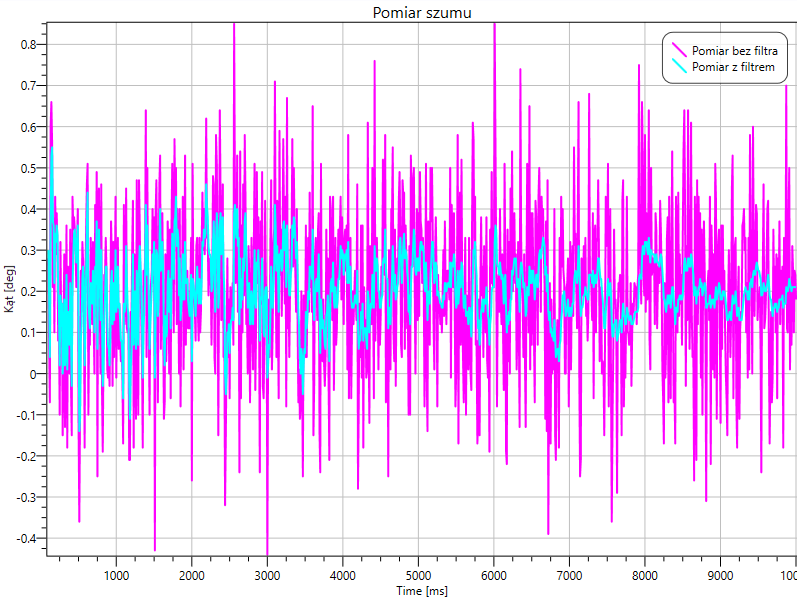
\includegraphics[width=0.48\textwidth]{pictures/theta_stand.png}
    }
    \hfill
    \subfloat[Szum dla $\phi$\label{subfig-6:tphi_stand}]
    {
      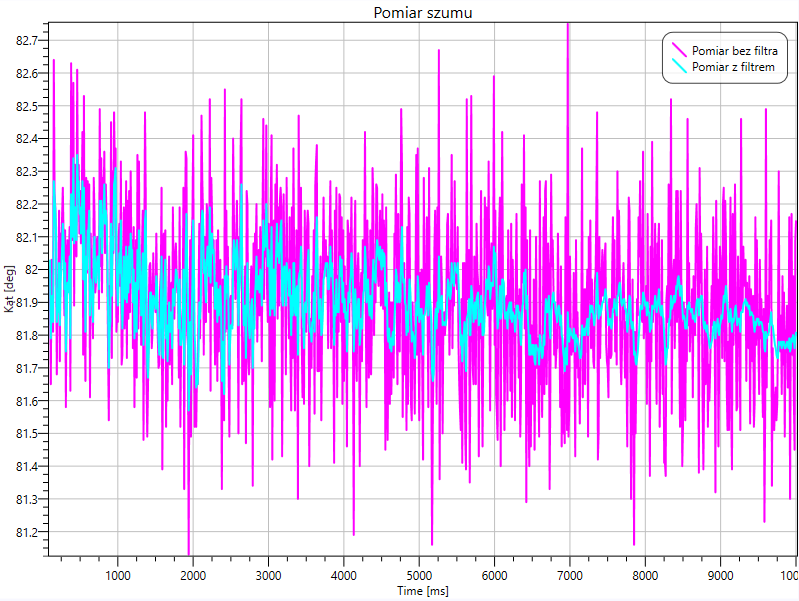
\includegraphics[width=0.48\textwidth]{pictures/phi_stand.png}
    }
    \caption{Charakterystyki czujnika: leżącego ((a) i (b)) i stojącego ((c) i (d))}
    \label{fig:szum_sit}
\end{figure}

Widać, że podane szumy w każdym z przypadków wprowadzają niepewność pomiarową wynoszącą $1^{o}$. Filtr zmniejsza ją do poziomu $0.5^{o}$. Jednak by ten zaczął poprawnie działać potrzebne jest kilkadziesiąt próbek by estymacja osiągała sensowne wartości.

\section{Pomiary laboratoryjne}

Moduł SEN0142 został zamocowany do elementu obrotowego silnika za pomocą kleju \emph{Kropelka}. Został on wytypowany na podstawie tego, że wiąże materiały na sztywno, tak więc czujnik nie będzie ciągnięty przez powierzchnię, na której się znajduje, a raczej stworzy z nią integralną całość. W pierwszej kolejności po przymocowaniu czujnika wykreślono jego szum:

\begin{figure}[H]
    \subfloat[Szum dla $\theta$\label{moc1}]
    {
      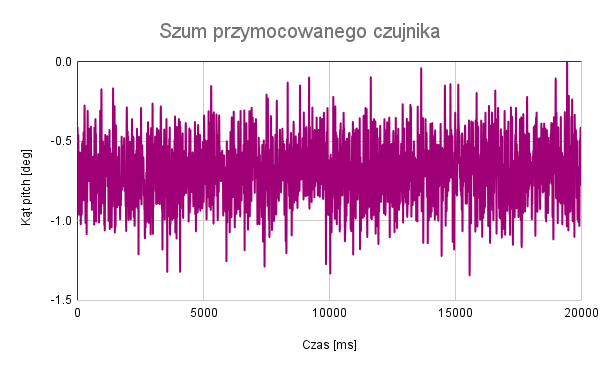
\includegraphics[width=0.48\textwidth]{pictures/szum_mocowanko.png}
    }
    \hfill
    \subfloat[Szum dla $\phi$\label{moc2}]
    {
      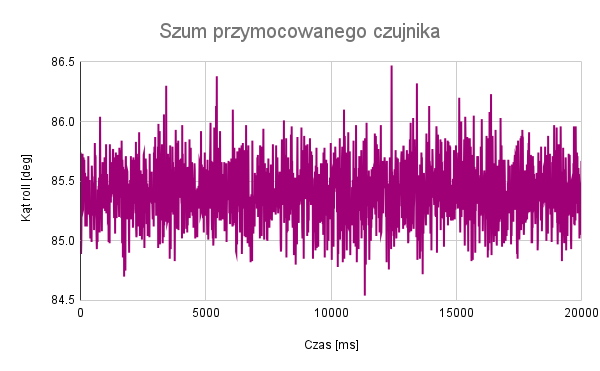
\includegraphics[width=0.48\textwidth]{pictures/szum_mocowanko_2.png}
    }
    \caption{Wykresy dla przymocowanego czujnika}
    \label{fig:szumu_szumu}
\end{figure}

Uśredniając pomiary wykorzystane do wykresów otrzymano wartości początkowe (wraz z ich odchyleniami standardowymi) w jakich ustawiony jest czujnik. Wyniosły one:

\begin{itemize}
    \item Kąt pitch $\theta = -0.69 \pm 0.19$ [deg]
    \item Kąt roll $\phi = 85.41 \pm 0.25$ [deg]
\end{itemize}

Widać, że wartości nie wynoszą idealnie $0^{o}$ i $90^{o}$. Biorąc pod uwagę, że sam LCT znajduje się w fazie prototypowej, należy uwzględnić błąd wynikający z ręcznego składania urządzenia (np. fakt, że samo zwierciadło nie jest idealnie wycentrowane).

Po włączeniu symulacji na tomografie i załączeniu pomiaru położenia w aplikacji, czujnik po kilku pomiarach zamilkł. W przypadku pomiaru zmiany kątów żyroskopem nie otrzymano żadnej odpowiedzi. 

\begin{table}[H]
    \centering
    \caption{Otrzymane wyniki podczas ruchu zwierciadła}
    \begin{tabular}{l|cccc}
        \toprule
            Czas [ms]  &     0 &    10 &     20 &     30 \\
            Pitch [deg] & 64.75 & 62.86 & -46.87 & -54.72 \\
            Roll [deg] & 24.61 & 24.63 &  25.09 &  23.43 \\
        \bottomrule
    \end{tabular}
    \label{tab:ruch_false}
\end{table}

\newpage

Po wykreśleniu dane przedstawiły się następująco:

\begin{figure}[H]
    \centering
    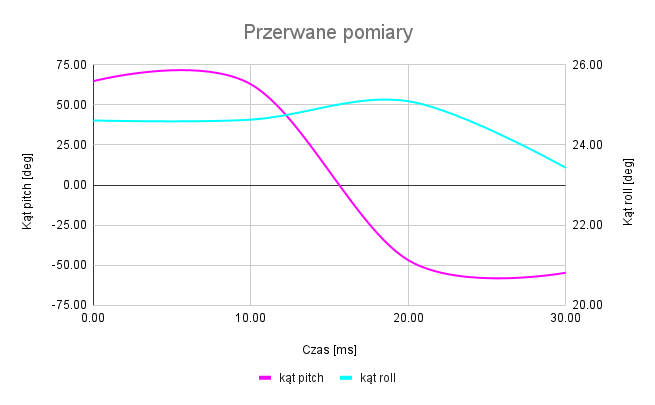
\includegraphics[width=\textwidth]{pictures/false.png}
    \caption{Nieukończone pomiary}
    \label{fig:false}
\end{figure}

Na charakterystyce kąta pitch widać, zapoczątkowanie ruchu okresowego, jednakże nic więcej nie da się z owej wizualizacji wywnioskować.

Potencjalnym źródłem błędów mogą być asymetryczne działanie momentów bezwładności wprowadzone przez przewody podłączone do czujnika. Przewody zostały ze sobą sklejone oraz usztywnione w odpowiednich miejscach, przyjęto więc wzór na moment bezwładności prętu o długości $l$ nachylonego do osi obrotu pod kątem $\alpha$.

\begin{equation}
    I = \frac{1}{3}ml^{2}\sin^{2}{\alpha}
\end{equation}

W celu wyznaczenia niepewności wykorzystano metodę różniczki zupełnej:

\begin{equation}
    \delta I = \Bigg|\frac{\partial I}{\partial m}\Bigg| \delta m + \Bigg|\frac{\partial I}{\partial l}\Bigg| \delta l + \Bigg|\frac{\partial I}{\partial \alpha}\Bigg| \delta \alpha
\end{equation}

Dane:
\begin{itemize}
    \item $m = 18 \pm 1$ [g],
    \item $l = 45.0 \pm 0.1$ [cm],
    \item $\alpha = 60^{o} \pm 5^{o}$
\end{itemize}

Moment bezwładności otrzymany wraz z niepewnością wyniósł:

$$
I = \frac{1}{3} \cdot 18 \cdot 45^{2} \cdot \sin^{2}{60} = 0.911 \pm 0.005 \; [kg \cdot m^{2}]
$$

Widać, że moment ten występuje, może więc on bezpośrednio zaburzać ruch masy w akcelerometrze, przez co czujnik przestaje odczytywać dane. Dodatkowo, przez ręczne zamontowanie elementów (zwierciadło, czujnik) elementy te nie są umieszczone idealnie symetrycznie, co w efekcie wprowadza asymetrię do rozkładu momentów bezwładności.
\chapter{PODSUMOWANIE I WNIOSKI KOŃCOWE}

Opracowane rozwiązanie okazało się niewystarczające. Pomimo spełniania teoretycznych założeń, w praktyce opracowany czujnik nie spełnia swojej funkcji. Wpływa na to parę czynników.

\begin{itemize}
    \item Czujnik przy dużych prędkościach przerywa pomiar, traci orientację w przestrzeni.
    \item Przewody łączące sensor SEN0142 z płytką Arduino wprowadzają dodatkowe zaburzenia:
    \begin{itemize}
        \item są to elementy posiadające masę, dodają więc dodatkowe obciążenie do układu, co przekłada się na zmiany momentów bezwładności elementu obrotowego silnika krokowego,
        \item przewody nie są trwale przyłączone (przylutowane, bądź zaciśnięte rurką termokurczliwą) do modułu SEN0142, nałożono jedynie złącza żeńskie na piny, może więc dochodzić do spadków napięcia, co zaburza prawidłową pracę czujnika.
    \end{itemize}
    \item Ograniczenie częstotliwości próbkowania do $100$ Hz niekorzystnie wpływa na jakość samego pomiaru.
    \item Silnik krokowy jest rozwiązaniem tymczasowym, ponieważ wymusza długi czas symulacji wykonywanej przez LCT. Rozważa się zastosowanie silnika rezonansowego, lub też skanera galwanometrycznego, które docelowo mają skrócić symulację. Czujnik, przez częstotliwość, na której pracuje, nie znajdzie zastosowania w owej technologii (jest zbyt ograniczony).
    \item Opracowane rozwiązanie miałoby zastosowanie przy badaniu obiektów powolnie zmieniających swoje położenie w przestrzeni. Przy prędkościach z jakimi porusza się silnik krokowy, czujnik obecnie nie jest przydatny.
\end{itemize}

Kolejnym ograniczającym rozwiązaniem było wykorzystanie \emph{Microsoft WPF}. Pomimo, że umożliwia łatwe i szybkie utworzenie aplikacji z graficznym interfejsem, blokuje ono wykorzystanie programu na innych systemach operacyjnych niż \emph{Microsoft Windows}. Jeśli aplikacja miałaby być multiplatformowa (potencjalnie z implementacją również na urządzeniach mobilnych) warto by było zastosować platformę do stworzenia aplikacji webowej (np. React.JS, Angular, Google Flutter), dzięki czemu zostałoby zniwelowane ograniczenie do jednej platformy. Co więcej, przy integracji z bazą danych, możliwe by było jednoczesne składowanie wcześniej wykonanych pomiarów.

Należałoby również wymienić moduł na taki, który posiada wbudowany przekaźnik bezprzewodowy. Zniwelowałoby to problem jakim są przewody, a raczej ich masa. Jednakże, w takim wypadku trzeba zagwarantować jak najmniejszą stratę danych.

Rozwiązaniem, które umożliwiłoby pracę czujnika na większych częstotliwościach, wymagałoby wykorzystania pamięci Arduino - skrypt zapisywałby pomiary na płytce, a dopiero potem przesyłał je do komputera. Byłoby to problematyczne o tyle, że tej jest relatywnie niewiele. Należałoby zastosować rozwiązanie technologiczne umożliwiające podłączenie dodatkowej pamięci, np. Raspberry Pi. Byłoby ono o tyle wygodne, że w odróżnieniu od Arduino, które jest jedynie płytką z mikrokontrolerem, jest to w pełni funkcjonalny komputer, z własnym systemem operacyjnym na jądrze Linuxa. Takie rozwiązanie byłoby rozsądniejsze o tyle, że samą aplikację sterującą można by zaimplementować już na Raspberry Pi. Dodatkowym atutem jest łatwiejsze programowanie - to bazuje na Bashu lub Pythonie.

\begin{figure}[H]
    \centering
    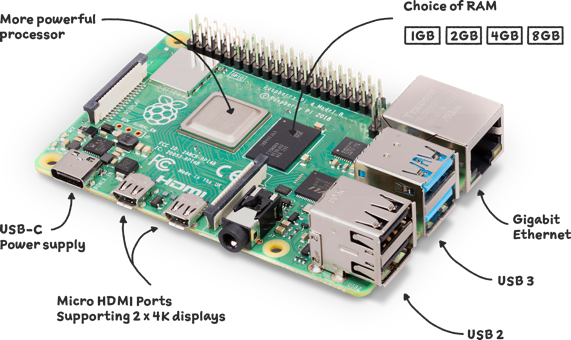
\includegraphics[width=\textwidth]{pictures/raspberry_pi_4.png}
    \caption{Komputer Raspberry Pi 4B \cite{pi}}
    \label{fig:rsp}
\end{figure}

Na rys. 5.1 widać, że zniknąłby problem z prędkością przesyłania danych, bo te byłyby bezpośrednio składowane na Raspberry Pi, lub też pamięci zewnętrznej podłączonej do tego komputera. Samo urządzenie ma wbudowane złącze Ethernet (dostęp do internetu w razie potrzeby jest więc zapewniony). Można je również skonfigurować z mocniejszym komputerem by działały w relacji master-slave. Wadą tego rozwiązania jest jednak cena zestawu - na przestrzeni ostatnich lat Raspberry Pi podrożało, gdyż zaczęto je wykorzystywać do kopania kryptowalut.



% ---------------------- Bibliografia -----------------------
\bibliographystyle{plain}
\begin{thebibliography}{3}
\addcontentsline{toc}{chapter}{Wykaz literatury}
\small

\bibitem{algo}
Kristy K. Brock, Sasa Mutic, Todd R. McNutt, Hua Li, Marc L. Kessler: \href{https://aapm.onlinelibrary.wiley.com/doi/10.1002/mp.12256}{\emph{Use of image registration and fusion algorithms and techniques in radiotherapy: Report of the AAPM Radiation Therapy Committee Task Group No. 132}}, (2017) Med. Phys. Volume 44, Issue 7, data dostępu: 06.01.2022 r.

\bibitem{image}
K. Sjogreen-Gleisner, D. Rueckert, M. Ljungberg: \href{https://iopscience.iop.org/article/10.1088/0031-9155/54/20/010/pdf}{\emph{Registration of serial SPECT/CT images for threedimensional dosimetry in radionuclide therapy}}, (2009) Physics in Medicine \& Biology, Volume 54, Number 20, data dostępu: 06.01.2022 r.

\bibitem{Mar}
M. Maryanski (2018), \emph{High-Definition 3D Dosimetry for End-To-End Patient-Specific Treatment Delivery Verification}. W: Chan Maria F., Editor, \emph{Recent Advancements and Applications in Dosimetry}. Wyd. Nova, ISBN: 978-1-53613-759-0.

\bibitem{inclino}
\href{https://www.mouser.pl/datasheet/2/281/1/datasheet_scl3300_d01-1532018.pdf}{Dokumentacja 3-osiowego inklinometru SCL3300-D01}, data dostępu: 04.01.2022 r.

\bibitem{filtr}
Dr inż. Marek Wnuk: \href{http://docplayer.pl/47112054-Katedra-cybernetyki-i-robotyki-wydzial-elektroniki.html}{\emph{Filtracja komplementarna w inercyjnych czujnikach orientacji}}, \\
Politechnika Wrocławska, Wrocław 2014, data dostępu: 12.12.2022 r.

\bibitem{kal}
Dr inż. Piotr Suchomski: \href{https://eti.pg.edu.pl/documents/176593/26524402/TS-5.pdf}{\emph{Liniowe filtry Kalmana}},
Politechnika Gdańska, data dostępu: 12.12.2022 r.

\bibitem{Ardocs}
\href{https://docs.arduino.cc/hardware/uno-rev3}{\emph{Oficjalna dokumentacja Arduino Uno}}, data dostępu: 12.12.2022 r.

\bibitem{shop}
\href{https://www.dfrobot.com/product-880.html}{\emph{Sklep producenta}}, data dostępu: 29.12.2022 r.

\bibitem{dfr}
\href{https://invensense.tdk.com/wp-content/uploads/2015/02/MPU-6000-Datasheet1.pdf}{\emph{MPU-6000 and MPU-6050 Product Specification Revision 3.4}}, InvenSense, Sunnyvale 2013, data dostępu: 12.12.2022 r.

\bibitem{forbot}
Forbot, \emph{Magistarala I2C}

\bibitem{csh}
\href{https://learn.microsoft.com/en-us/dotnet/api/system.threading.thread?view=net-7.0}{\emph{Dokumentacja języka C\# i platformy .NET}}, data dostępu: 20.12.2022 r.

\bibitem{pi}
\href{https://www.raspberrypi.com/products/raspberry-pi-4-model-b/}{\emph{Oficjalna strona rozwiązania Raspberry Pi}}, data dostępu: 29.12.2022 r.
\end{thebibliography}
% -----------------------------------------------------------

%------------------------------------------------------------
%	Dodanie wykazu rysunków oraz tabeli

\renewcommand{\baselinestretch}{1.0}\normalsize
\addcontentsline{toc}{chapter}{\listfigurename}
\listoffigures

\renewcommand{\baselinestretch}{1.0}\normalsize
\addcontentsline{toc}{chapter}{Wykaz listingów}
\listof{lstlisting}{Wykaz listingów}

\addcontentsline{toc}{chapter}{\listtablename}
\listoftables
\renewcommand{\baselinestretch}{1.3}\normalsize

% ---------------------- DODATKI -----------------------
\chapter*{Dodatki}
\addcontentsline{toc}{chapter}{Dodatki}
% Zaleznie od dodatku, zaleca sie dodawac dodatki jako
% dokumenty PDF
% \includepdf{dodatki/dodatek1.pdf}

Poniżej znajdują sią kody źródłowe opracowanego rozwiązania, pełne projekty dostępne na:
\begin{itemize}
    \item Arduino: \url{https://github.com/StachRach/dyplom-arduino-final.git}
    \item Aplikacja: \url{https://github.com/StachRach/dyplom-WPF.git}
\end{itemize}

\lstinputlisting[caption=Skrypt Arduino, language=c++, firstline=6]{listings/main.cpp}
\lstinputlisting[caption=Klasa aplikacji, language=csh, firstline=6]{listings/MainWindow2.xaml.cs}
\lstinputlisting[caption=Formularz XAML aplikacji, language=xml, firstline=6]{listings/MainWindow.xaml}

% -----------------------------------------------------------
\end{document}
%------------------------------------------------------------
			 	%	Koniec pracy dyplomowej  %
%------------------------------------------------------------
